\clearpage

\section{Simulation Analysis}
\label{sec:simulation}

In Figure \ref{fig:circuit-ngspice}, the circuit used by \textit{Ngspice} is displayed. Instead of the transformer, we use one voltage controlled volateg source and one current controlled current source to simulate an ideal transformer. Furthermore, we add a 0V voltage source between nodes 2 and 4 because \textit{Ngspice} needs it for the current source to work. Moreover, the diodes used are the default ones created by the \textit{software}.

\begin{figure}[h] \centering
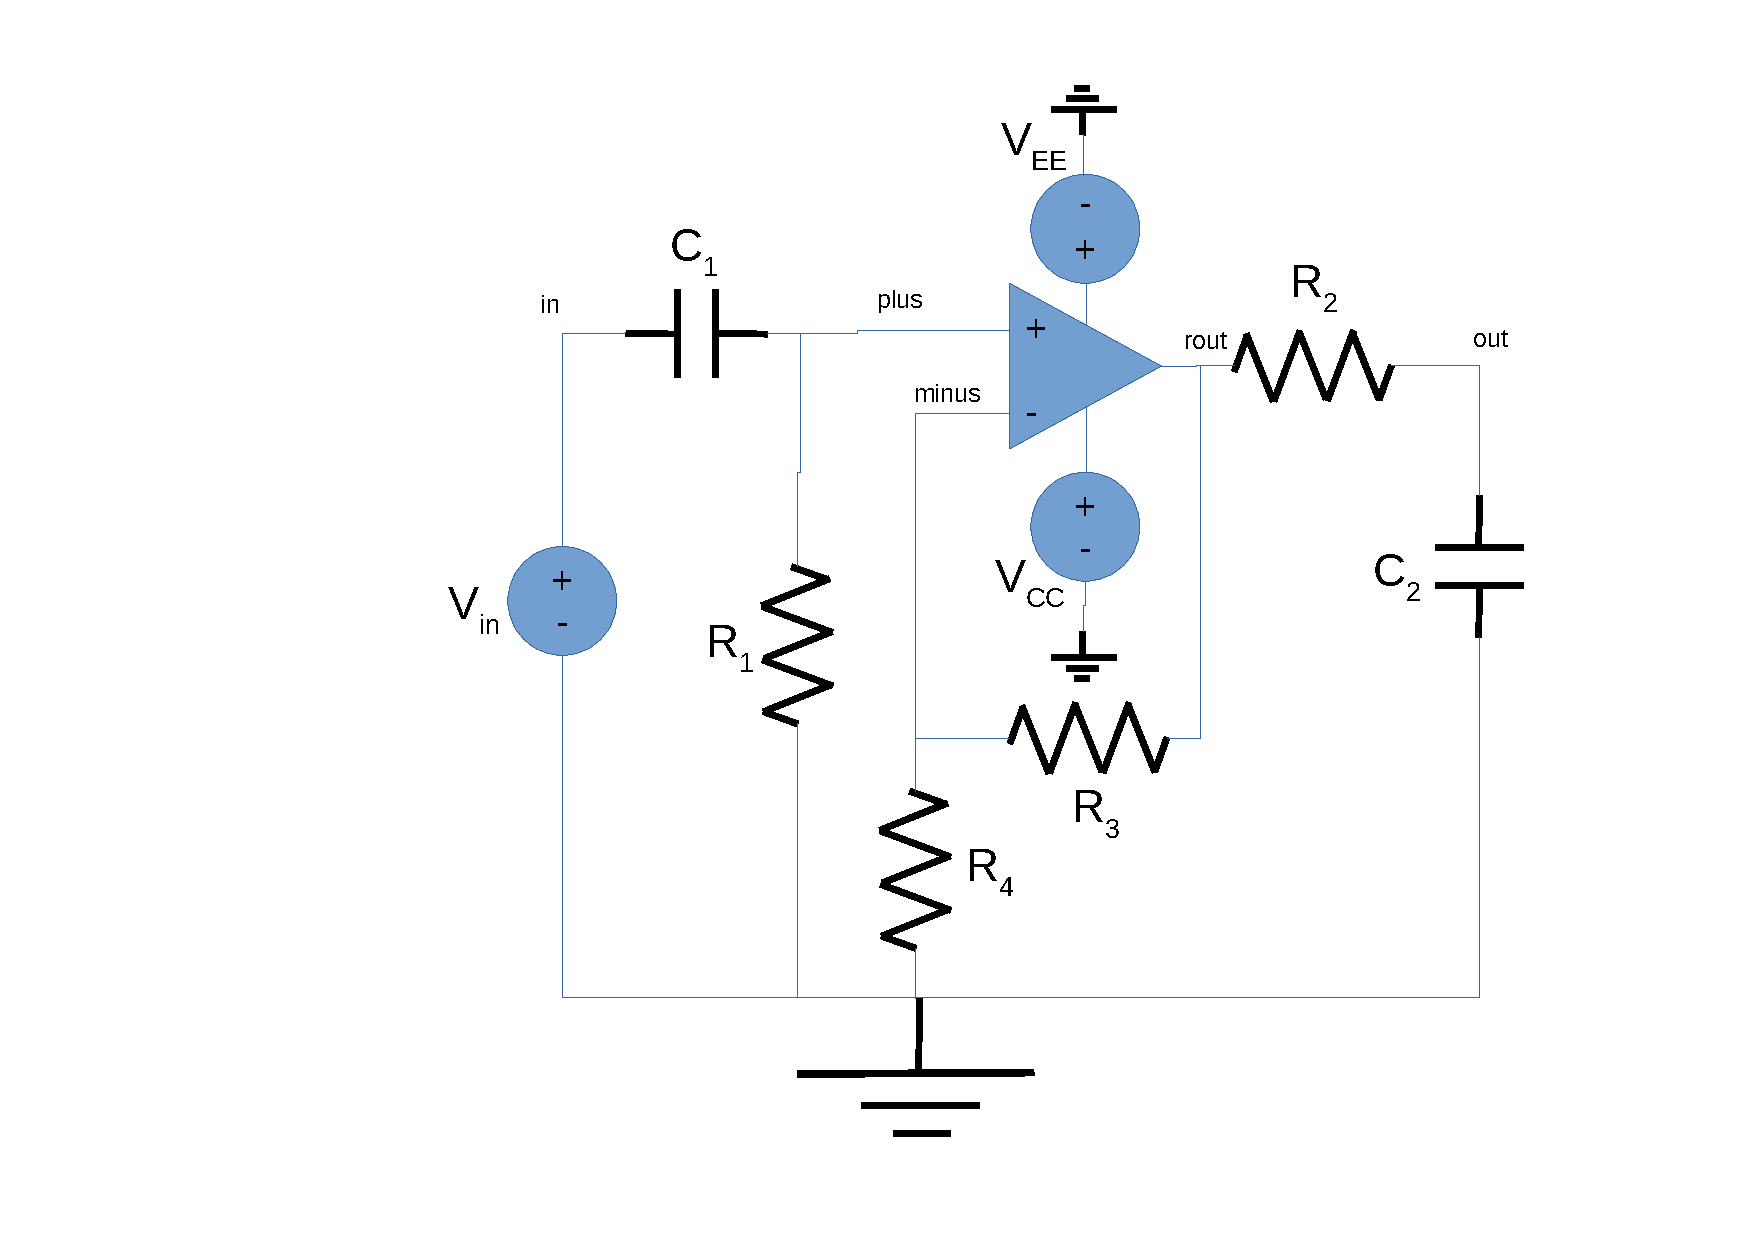
\includegraphics[width=0.6\linewidth]{circuit.pdf}
\caption{The circuit we will be working with.}
\label{fig:circuit-ngspice}
\end{figure}